\documentclass[12pt, twoside]{article}
\usepackage[letterpaper, margin=1in, headsep=0.5in]{geometry}
\usepackage[english]{babel}
\usepackage[utf8]{inputenc}
\usepackage{amsmath}
\usepackage{amsfonts}
\usepackage{amssymb}
\usepackage{tikz}

\usepackage{pgfplots}
\pgfplotsset{width=9cm,compat=1.9}

\usepackage{venndiagram}

\usepackage{graphicx}
\usepackage{enumitem}
\usepackage{multicol}

\usepackage{fancyhdr}
\pagestyle{fancy}
\fancyhf{}
\renewcommand{\headrulewidth}{0pt} % disable the underline of the header

\fancyhead[LE]{\thepage}
\fancyhead[RO]{\thepage \\ Name: \hspace{4cm} \,\\}
\fancyhead[LO]{BECA / Dr. Huson / IB Mathematics\\* Unit 4: Linear functions and regression\\* 17 January 2020}

\begin{document}
\begin{enumerate}
    \subsubsection*{4.11 Exam: Linear equations, function operations, regression}

    \item {[Maximum mark: 9]} \\[0.3cm]
    The diagram shows the straight line $L_1$, which intersects the $x$-axis at $A(k, 0)$ and the $y$-axis at $B(0,8)$. The gradient of $L_1$ is $-\frac{2}{3}$. \hfill \emph{Diagram is not to scale}
        \begin{center}
            \begin{tikzpicture}[scale=1]
            %\draw [help lines] (0,0) grid (10,8);
            \draw [thick, ->] (-0.5,0) -- (7.4,0) node [below right] {$x$};
            \draw [thick, ->] (0,-0.5)--(0,3.4) node [left] {$y$};
            %\draw [fill] (9,5) circle [radius=0.1];
            \draw [thick, -] (-0.25,3) node [below] {$B$}--(6,-0.1) node [above] {$A$};
            \end{tikzpicture}
        \end{center}
        \begin{enumerate}%[itemsep=3cm]
            \item Find the value of $k$. \hfill [2]
            \item Write down the coordinates of the midpoint $M$ of $A$ and $B$. \hfill [2]
            \item Write down the equation for the line $L_1$. \hfill [2]
            \item The line $L_2$ is perpendicular to $L_1$ and passes through $M$. \hfill [3]\\[0.2cm]
            Find the equation for the line $L_2$.
        \end{enumerate}
        \begin{tikzpicture}
            \draw (0,0) rectangle (15.5,11);
            \draw [dotted] (1,10)--(14,10);
            \draw [dotted] (1,9)--(14,9);
            \draw [dotted] (1,8)--(14,8);
            \draw [dotted] (1,7)--(14,7);
        \end{tikzpicture}

\newpage 
    \item {[Maximum mark: 7]} \\[0.3cm]
    Let $f(x)=3x+7$ and $g(x)=5x$, for $x \in R$.
        \begin{enumerate}
            \item Write down $g(2)$. \hfill [1]
            \item Find $(f \times g)(x)$. \hfill [1]
            \item Find $(f \circ g)(x)$. \hfill [1]
            \item Write down $g^{-1}(10)$. \hfill [2]
            \item Find $f^{-1}(x)$. \hfill [2]
        \end{enumerate}
        \begin{tikzpicture}
            \draw (0,-4) rectangle (15.5,11);
            \draw [dotted] (1,10)--(14,10);
            \draw [dotted] (1,9)--(14,9);
            \draw [dotted] (1,8)--(14,8);
            \draw [dotted] (1,7)--(14,7);
            \draw [dotted] (1,6)--(14,6);
        \end{tikzpicture}

\newpage
   \item {[Maximum mark: 6]} \\[0.3cm]
   Early finishers: The diagram below shows the graph of a function $f$ for $-2 \leq x \leq 3$. 
        \begin{center}
        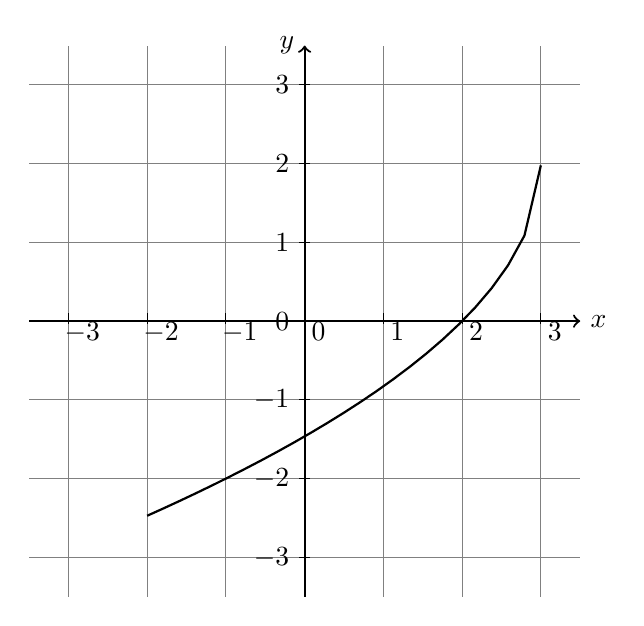
\begin{tikzpicture}[scale=1.0]
                \draw [thin, color=gray, xstep=1.0cm,ystep=1.0cm] (-3.5,-3.5) grid (3.5,3.5);
                %\draw [thin, color=lightgray,, xstep=0.2cm,ystep=0.2cm] (-5.5,-4.5) grid (5.5,6.5);
                \foreach \x in {-3, -2, -1, 0,1,2,3}
                    \draw[shift={(\x,0)},color=black] (0pt,-1pt) -- (0pt,3pt) node[below]  {$\quad \x$};
                \foreach \y in {-3, -2,-1,0,1,2,3}
                    \draw[shift={(0,\y)},color=black] (2pt,0pt) -- (-2pt,0pt) node[left]  {$\y$};
                \draw [thick, ->] (-3.5,0) -- (+3.5,0) node [right] {$x$};
                \draw [thick, ->] (0,-3.5) -- (0,3.5) node [left] {$y$};
            \draw [thick] plot[domain= -2:3] (\x, {-2*(-\x+3)^0.5 +2});
            %\draw [thick] plot[domain= -1:2] (\x, \x*1/2 -2);
            %\draw [thick] (-2,-2).. controls (0,-1) and (2,0) .. (3,1);
            %\draw [fill] (-3,3) circle[radius=0.1] node[above left]{$A(-3,3)$};
        \end{tikzpicture}
        \end{center}
        \begin{enumerate}%[itemsep=2cm]
            \item Write down the value of $f(2)$. \hfill [1]
            \item Write down the value of $f^{-1}(-2)$. \hfill [2]
            \item Sketch the graph of $f^{-1}$ on the grid. \hfill [3]
        \end{enumerate}
        \begin{tikzpicture}
            \draw (0,1) rectangle (15.5,11);
            \draw [dotted] (1,10)--(14,10);
            \draw [dotted] (1,9)--(14,9);
            \draw [dotted] (1,8)--(14,8);
            \draw [dotted] (1,7)--(14,7);
            \draw [dotted] (1,6)--(14,6);
        \end{tikzpicture}

\newpage
    \item  {[Maximum mark: 6]} \\[0.3cm]
        The North Carolina Research Triangle is one of the world's leading regions for high tech businesses and research. The three universities that anchor the area, Duke University, University of North Carolina at Chapel Hill, and North Carolina State University, form a triangle as shown below. \\[0.25cm]
        Assume that the distance from UNCC to NC State is 40 km, from UNCC to Duke is 16 km, and that the angle made by Duke, UNCC, and NC State is $64^\circ$.
        \begin{center}
        \begin{tikzpicture}[scale=1.2]
            \draw [-, thick] (40:3) node[above right]{Duke}--
            (0,0) node[left]{UNCC}--
            (-25:7) node[right]{NC State}--cycle;
            \draw (-25:0.9) arc (-25:40:0.9);
            \node at (0.2, 0.1)[right]{$64^\circ$};
            \node at (-30:4)[above left]{40 km};
            \node at (65:1.8)[below]{16 km};
        \end{tikzpicture}
        \end{center} 
        \begin{enumerate}
            \item Calculate the distance from Duke to NC State. \hfill [3]
            \item Find the area of the triangle formed by the three universities. \hfill [3]
        \end{enumerate}
        \begin{tikzpicture}
            \draw (0,0) rectangle (15.2,8);
            \draw (8,0) rectangle (15.2,3);
            \node at (0,8)[below right]{\textbf{Working:}};
            \node at (8,3)[below right]{\textbf{Answers:}};
            \draw [dotted] (9,1.7)node[left]{(a)}--(15,1.7);
            \draw [dotted] (9,1)node[left]{(b)}--(15,1);
        \end{tikzpicture}

\end{enumerate}
\end{document}